\ifx\wholebook\relax \else
% ------------------------

\documentclass{article}
%------------------- Other types of document example ------------------------
%
%\documentclass[twocolumn]{IEEEtran-new}
%\documentclass[12pt,twoside,draft]{IEEEtran}
%\documentstyle[9pt,twocolumn,technote,twoside]{IEEEtran}
%
%-----------------------------------------------------------------------------
%%
% loading packages
%
\newif\ifpdf
\ifx\pdfoutput\undefined % We're not running pdftex
  \pdffalse
\else
  \pdftrue
\fi
%
%
\ifpdf
  \RequirePackage[pdftex,%
            CJKbookmarks,%
       bookmarksnumbered,%
              colorlinks,%
          linkcolor=blue,%
              hyperindex,%
        plainpages=false,%
       pdfstartview=FitH]{hyperref}
\else
  \RequirePackage[dvipdfm,%
             CJKbookmarks,%
        bookmarksnumbered,%
               colorlinks,%
           linkcolor=blue,%
               hyperindex,%
         plainpages=false,%
        pdfstartview=FitH]{hyperref}
  \AtBeginDvi{\special{pdf:tounicode GBK-EUC-UCS2}} % GBK -> Unicode
\fi
\usepackage{hyperref}

% other packages
%-----------------------------------------------------------------------------
\usepackage{graphicx, color}
\usepackage{CJK}
%
% for programming 
%
\usepackage{verbatim}
\usepackage{listings}


\lstdefinelanguage{Smalltalk}{
  morekeywords={self,super,true,false,nil,thisContext}, % This is overkill
  morestring=[d]',
  morecomment=[s]{"}{"},
  alsoletter={\#:},
  escapechar={!},
  literate=
    {BANG}{!}1
    {UNDERSCORE}{\_}1
    {\\st}{Smalltalk}9 % convenience -- in case \st occurs in code
    % {'}{{\textquotesingle}}1 % replaced by upquote=true in \lstset
    {_}{{$\leftarrow$}}1
    {>>>}{{\sep}}1
    {^}{{$\uparrow$}}1
    {~}{{$\sim$}}1
    {-}{{\sf -\hspace{-0.13em}-}}1  % the goal is to make - the same width as +
    %{+}{\raisebox{0.08ex}{+}}1		% and to raise + off the baseline to match -
    {-->}{{\quad$\longrightarrow$\quad}}3
	, % Don't forget the comma at the end!
  tabsize=2
}[keywords,comments,strings]

\lstloadlanguages{C++, Lisp, Smalltalk}

% ======================================================================

\def\BibTeX{{\rm B\kern-.05em{\sc i\kern-.025em b}\kern-.08em
    T\kern-.1667em\lower.7ex\hbox{E}\kern-.125emX}}

\newtheorem{theorem}{Theorem}

%
% mathematics
%
\newcommand{\be}{\begin{equation}}
\newcommand{\ee}{\end{equation}}
\newcommand{\bmat}[1]{\left( \begin{array}{#1} }
\newcommand{\emat}{\end{array} \right) }
\newcommand{\VEC}[1]{\mbox{\boldmath $#1$}}

% numbered equation array
\newcommand{\bea}{\begin{eqnarray}}
\newcommand{\eea}{\end{eqnarray}}

% equation array not numbered
\newcommand{\bean}{\begin{eqnarray*}}
\newcommand{\eean}{\end{eqnarray*}}

\RequirePackage{CJK,CJKnumb,CJKulem,CJKpunct}
% we use CJK as default environment
\AtBeginDocument{\begin{CJK*}{GBK}{song}\CJKtilde\CJKindent\CJKcaption{GB}}
\AtEndDocument{\clearpage\end{CJK*}}

%
% loading packages
%
\newif\ifpdf
\ifx\pdfoutput\undefined % We're not running pdftex
  \pdffalse
\else
  \pdftrue
\fi
%
%
\ifpdf
  \RequirePackage[pdftex,%
       bookmarksnumbered,%
              colorlinks,%
          linkcolor=blue,%
              hyperindex,%
        plainpages=false,%
       pdfstartview=FitH]{hyperref}
\else
  \RequirePackage[dvipdfm,%
        bookmarksnumbered,%
               colorlinks,%
           linkcolor=blue,%
               hyperindex,%
         plainpages=false,%
        pdfstartview=FitH]{hyperref}
\fi
\usepackage{hyperref}

% other packages
%-----------------------------------------------------------------------------
\usepackage{graphicx, color}
%
% for programming 
%
\usepackage{verbatim}
\usepackage{listings}
\usepackage{algorithmic} %for pseudocode
\usepackage{algorithm}


\lstdefinelanguage{Smalltalk}{
  morekeywords={self,super,true,false,nil,thisContext}, % This is overkill
  morestring=[d]',
  morecomment=[s]{"}{"},
  alsoletter={\#:},
  escapechar={!},
  literate=
    {BANG}{!}1
    {UNDERSCORE}{\_}1
    {\\st}{Smalltalk}9 % convenience -- in case \st occurs in code
    % {'}{{\textquotesingle}}1 % replaced by upquote=true in \lstset
    {_}{{$\leftarrow$}}1
    {>>>}{{\sep}}1
    {^}{{$\uparrow$}}1
    {~}{{$\sim$}}1
    {-}{{\sf -\hspace{-0.13em}-}}1  % the goal is to make - the same width as +
    %{+}{\raisebox{0.08ex}{+}}1		% and to raise + off the baseline to match -
    {-->}{{\quad$\longrightarrow$\quad}}3
	, % Don't forget the comma at the end!
  tabsize=2
}[keywords,comments,strings]

\lstloadlanguages{C++, Lisp, Haskell, Python, Smalltalk}

% ======================================================================

\def\BibTeX{{\rm B\kern-.05em{\sc i\kern-.025em b}\kern-.08em
    T\kern-.1667em\lower.7ex\hbox{E}\kern-.125emX}}

\newtheorem{theorem}{Theorem}

%
% mathematics
%
\newcommand{\be}{\begin{equation}}
\newcommand{\ee}{\end{equation}}
\newcommand{\bmat}[1]{\left( \begin{array}{#1} }
\newcommand{\emat}{\end{array} \right) }
\newcommand{\VEC}[1]{\mbox{\boldmath $#1$}}

% numbered equation array
\newcommand{\bea}{\begin{eqnarray}}
\newcommand{\eea}{\end{eqnarray}}

% equation array not numbered
\newcommand{\bean}{\begin{eqnarray*}}
\newcommand{\eean}{\end{eqnarray*}}




\setcounter{page}{1}

\begin{document}

%--------------------------

% ================================================================
%                 COVER PAGE
% ================================================================

\title{Suffix Tree}

\author{Larry~LIU~Xinyu
\thanks{{\bfseries Larry LIU Xinyu } \newline
  Email: liuxinyu95@gmail.com \newline}
  }

\maketitle
\fi

\markboth{Suffix Tree}{Elementary Algorithms}

\ifx\wholebook\relax
\chapter{Suffix Tree}
\numberwithin{Exercise}{chapter}
\fi

%{\bfseries Corresponding Author:} Larry LIU Xinyu

% ================================================================
%                 Introduction
% ================================================================
\section{Introduction}
\label{introduction}
\index{Suffix tree}

Suffix Tree is an important data structure.
It can be used to realize many important string operations particularly
fast\cite{wiki-suffix-tree}. It is
also widely used in bio-information area such as DNA pattern
matching\cite{ukkonen-presentation}.
Weiner introduced suffix tree in 1973\cite{weiner73}.
The latest on-line construction algorithm was found in 1995\cite{ukkonen95}.

The suffix tree for a string $S$ is a special Patricia.
Each edge is labeled with some sub-string of $S$.
Each suffix of $S$ corresponds to exactly one path
from the root to a leaf. Figure \ref{fig:stree-banana} shows the suffix tree for
English word `banana'.

\begin{figure}[htbp]
  \centering
  \includegraphics[scale=0.5]{img/stree-banana.ps}
  \caption{The suffix tree for `banana'} \label{fig:stree-banana}
\end{figure}

All suffixes, 'banana', 'anana', 'nana', 'ana', 'na', 'a', '' can
be found in the above tree. Among them the first 3 suffixes are explicitly
shown; others are implicitly represented. The reason for why 'ana, 'na', 'a',
and '' are not shown is because they are prefixes of the others.
In order to show all suffixes explicitly, we can append a special pad
terminal symbol, which doesn't occur in other places in the string.
Such terminator is typically
denoted as '\$'. By this means, there is no suffix being the prefix of the others.

Although the suffix tree for 'banana' is simple, the
suffix tree for 'bananas', as shown in figure \ref{fig:stree-bananas}, is quite different.

\begin{figure}[htbp]
  \centering
  \includegraphics[scale=0.5]{img/stree-bananas.ps}
  \caption{The suffix tree for `bananas'} \label{fig:stree-bananas}
\end{figure}

To create suffix suffix tree for a given string, we can utilize the
insertion algorithm explained in previous chapter for Patricia.

\begin{algorithmic}[1]
\Function{Suffix-Tree}{$S$}
  \State $T \gets$ NIL
  \For{$i \gets 1$ to $|S|$}
    \State $T \gets$ \textproc{Patricia-Insert}($T$, \Call{Right}{$S, i$})
  \EndFor
  \State \Return $T$
\EndFunction
\end{algorithmic}

For non-empty string $S=s_1s_2...s_i...s_n$ of length $n = |S|$, function
\textproc{Right}($S, i$) $= s_is_{i+1...s_n}$. It extracts the sub-string of $S$
from the $i$-th character to the last one. This straightforward algorithm
can also be defined as below.

\be
suffix_T(S) = fold(insert_{Patricia}, \phi, suffixes(S))
\ee

Where function $suffixes(S)$ gives all the suffixes for string $S$. If
the string is empty, the result is one empty string; otherwise, $S$
itself is one suffix, the others can be given by recursively call
$suffixes(S')$, where $S'$ is given by drop the first character from $S$.

\be
suffixes(S) = \left \{
  \begin{array}
  {r@{\quad:\quad}l}
  \{ \phi \} & S = \phi \\
  \{S\} \cup suffixes(S') & otherwise
  \end{array}
\right.
\ee

This solution constructs suffix tree in $O(n^2)$ time, for string of length $n$.
It totally inserts $n$ suffixes to the tree, and each
insertion takes linear time proportion to the length of the suffix.
The efficiency isn't good enough.

In this chapter, we firstly explain a fast on-line suffix trie construction
solution by using suffix link concept. Because trie isn't space efficient,
we next introduce a linear time on-line suffix tree construction algorithm
found by Ukkonen. and show
how to solve some interesting string manipulation problems with
suffix tree.

% ================================================================
%                 Suffix Trie
% ================================================================
\section{Suffix trie}
\label{suffix-trie}
\index{Suffix trie}

Just likes the relationship between trie and Patricia, Suffix trie has much simpler
structure than suffix tree. Figure \ref{fig:strie-banana} shows the suffix trie for
'banana'.

\begin{figure}[htbp]
  \centering
  \includegraphics[scale=0.4]{img/strie-banana.ps}
  \caption{Suffix trie for 'banana'} \label{fig:strie-banana}
\end{figure}

Compare with figure \ref{fig:stree-banana}, we can find the difference between
suffix tree and suffix trie. Instead of representing
a word, every edge in suffix trie only represents a character.
Thus suffix trie needs much more spaces.
If we pack all nodes which have only one child, the suffix
trie is turned into a suffix tree.

We can reuse the trie definition for suffix tree. Each node is bound to a
character, and contains multiple sub trees as children. A child can be
referred from the bounded character.

% ================================================================
%               Online construction of Suffix Trie
% ================================================================
\subsection{Node transfer and suffix link}

For string $S$ of length $n$, define $S_i=s_1s_2...s_i$.
It is the prefix contains the first $i$ characters.

\index{Suffix tree!node transfer}
In suffix trie, each node represents a suffix string. for example in figure
\ref{fig:strie-cacao}, node $X$ represents suffix 'a', by adding character 'c',
node $X$ transfers to $Y$ which represents suffix 'ac'. We say node $X$ transfer
to $Y$ with the edge of character 'c'\cite{ukkonen95}.

\begin{figure}[htbp]
  \centering
  \includegraphics[scale=0.45]{img/strie-cacao.ps}
  \caption{Suffix trie for string ``cacao''. Node $X \gets$ ``a'', node $Y \gets$ ``ac'', $X$ transfers to $Y$ with character 'c'}
  \label{fig:strie-cacao}
\end{figure}

\begin{algorithmic}
\State $Y \gets$ \Call{Children}{$X$}[$c$]
\end{algorithmic}

We also say that node $X$ has a 'c'-child $Y$. Below Python expression
reflects this concept.

\lstset{language=python}
\begin{lstlisting}
y = x.children[c]
\end{lstlisting}

\index{Suffix link}
If node $A$ in a suffix trie represents suffix $s_is_{i+1}...s_n$,
and node $B$ represents suffix $s_{i+1}s_{i+2}...s_n$, we say node $B$
represents {\em the suffix} of node $A$. We can create a link from $A$ to $B$.
This link is defined as {\em the suffix link} of node $A$\cite{ukkonen95}.
Suffix link is drawn in dotted style. In figure \ref{fig:strie-cacao}, the suffix link of
node $A$ points to node $B$, and the suffix link of node $B$ points to node $C$.

Suffix link is valid for all nodes except the root. We can add a suffix link field to
the trie definition. Below Python example code shows this update.

\lstset{language=Python}
\begin{lstlisting}
class STrie:
    def __init__(self, suffix=None):
        self.children = {}
        self.suffix = suffix
\end{lstlisting}

\subsection{On-line construction}
\index{Suffix trie!on-line construction}

For string $S$, Suppose we have constructed suffix trie for the $i$-th prefix
$S_i=s_1s_2...s_i$. Denote it as $SuffixTrie(S_i)$.
Let's consider how to obtain $SuffixTrie(S_{i+1})$ from $SuffixTrie(S_i)$.

If list all suffixes corresponding to $SuffixTrie(S_i)$, from the longest
(which is $S_i$) to the shortest (which is empty), we can get
table \ref{tab:suffixes_s_i}. There are total $i+1$ suffixes.

\begin{table}
  \begin{tabular}{r}
    suffix string \\
    $s_1s_2s_3...s_i$ \\
    $s_2s_3...s_i$ \\
    ... \\
    $s_{i-1}s_i$ \\
    $s_i$ \\
    ``'' \\
  \end{tabular}
  \caption{suffixes for $S_i$}
  \label{tab:suffixes_s_i}
\end{table}

One solution is to append the character $s_{i+1}$ to every suffix in this
table, then add another empty string. This idea can be realized by adding
a new child for every node in the trie, and binding all these new
child with edge of character $s_{i+1}$.

\begin{algorithm}
\begin{algorithmic}[1]
\For{$\forall T \in SuffixTrie(S_i)$}
  \State \Call{Children}{$T$}[$s_{i+1}$] $\gets$ \Call{Create-Empty-Node}{}
\EndFor
\end{algorithmic}
\caption{Update $SuffixTrie(S_i)$ to $SuffixTrie(S_{i+1})$, initial version.}
\label{algo:strie1}
\end{algorithm}

However, some nodes in $SuffixTrie(S_i)$ may have the $s_{i+1}$-child already.
For example, in figure \ref{fig:strie-cac}, node $X$ and $Y$ are corresponding
for suffix 'cac' and 'ac' respectively. They don't have the 'a'-child.
But node $Z$, which represents suffix 'c' has the 'a'-child already.

\begin{figure}[htbp]
  \centering
  \subfloat[Suffix trie for string ``cac''.]{\hspace{.2\textwidth}\includegraphics[scale=0.5]{img/strie-cac.ps}\hspace{.2\textwidth}}
  \subfloat[Suffix trie for string ``caca''.]{\hspace{.2\textwidth}\includegraphics[scale=0.5]{img/strie-caca.ps}\hspace{.2\textwidth}}
  \caption{Suffix Trie of ``cac'' and ``caca''}
  \label{fig:strie-cac}
\end{figure}

When append $s_{i+1}$ to $SuffixTrie(S_i)$. In this example $s_{i+1}$ is character 'a'.
We need create new nodes for $X$ and $Y$, but we needn't do this
for $Z$.

If check the nodes one by one according to table \ref{tab:suffixes_s_i}, we can
stop immediately when meet a node which has the $s_{i+1}$-child. This is because
if node $X$ in $SuffixTrie(S_i)$ has the $s_{i+1}$-child, according to the
definition of suffix link, any suffix nodes $X'$ of $X$ in $SuffixTrie(S_i)$ must
also have the $s_{i+1}$-child. In other words, let $c=s_{i+1}$, if $wc$ is a sub-string
of $S_i$, then every suffix of $wc$ is also a sub-string of $S_i$ \cite{ukkonen95}.
The only exception is the root, which represents for empty string ``''.

According to this fact, we can refine the algorithm \ref{algo:strie1} to
the following.

\begin{algorithm}
  \begin{algorithmic}[1]
  \For{each $T \in SuffixTrie(S_i)$ in descending order of suffix length}
    \If{\Call{Children}{$T$}[$s_{i+1}$] = NIL}
      \State \Call{Children}{$T$}[$s_{i+1}$] $\gets$ \Call{Create-Empty-Node}{}
    \Else
      \State break
    \EndIf
  \EndFor
  \end{algorithmic}
  \caption{Update $SuffixTrie(S_i)$ to $SuffixTrie(S_{i+1})$, second version.}
  \label{algo:strie2}
\end{algorithm}

The next question is how to iterate all nodes
in descending order of the suffix length? Define the {\em top} of a suffix
trie as the deepest leaf node. This definition ensures the top represents
the longest suffix. Along the suffix link from the top to the next node,
the length of the suffix decrease by one. This fact tells us that
We can traverse the suffix tree from the top
to the root by using the suffix links. And the order of such traversing
is exactly what we want.
Finally, there is a special suffix trie for empty string $SuffixTrie(NIL)$,
We define the top equals to the root in this case.

\begin{algorithmic}
\Function{Insert}{$top, c$}
  \If{$top = $ NIL} \Comment{The trie is empty}
    \State $top \gets$ \Call{Create-Empty-Node}{}
  \EndIf
  \State $T \gets top$
  \State $T' \gets$ \Call{Create-Empty-Node}{} \Comment{dummy init value}
  \While{$T \neq$ NIL $\land$ \Call{Children}{$T$}[$c$] = NIL}
    \State \Call{Children}{$T$}[$c$] $\gets$ \Call{Create-Empty-Node}{}
    \State \Call{Suffix-Link}{$T'$} $\gets$ \Call{Children}{$T$}[$c$]
    \State $T' \gets$ \Call{Children}{$T$}[$c$]
    \State $T \gets$ \Call{Suffix-Link}{$T$}
  \EndWhile
  \If{$T \neq$ NIL}
    \State \Call{Suffix-Link}{$T'$} $\gets$ \Call{Children}{$T$}[$c$]
  \EndIf
  \State \Return \Call{Children}{$top$}[$c$] \Comment{returns the new top}
\EndFunction
\end{algorithmic}

Function \textproc{Insert}, updates $SuffixTrie(S_i)$ to $SuffixTrie(S_{i+1})$.
It takes two arguments, one is the top of $SuffixTrie(S_i)$, the other
is $s_{i+1}$ character. If the top is NIL, it means the tree is empty,
so there is no root. The algorithm creates a root node in this case.
A sentinel empty node $T'$ is created. It keeps tracking the previous
created new node. In the main loop, the algorithm checks every node
one by one along the suffix link. If the node hasn't the $s_{i+1}$-child,
it then creates a new node, and binds the edge to character $s_{i+1}$.
The algorithm repeatedly goes up along the suffix link until either
arrives at the root, or find a node which has the $s_{i+1}$-child already.
After the loop, if the node isn't empty, it means we stop at a node
which has the $s_{i+1}$-child.
The last suffix link then points to that child.
Finally, the new top position is returned, so that we can further
insert other characters to the suffix trie.

For a given string $S$, the suffix trie can be built by repeatedly
calling \textproc{Insert} function.

\begin{algorithmic}[1]
\Function{Suffix-Trie}{$S$}
  \State $t \gets$ NIL
  \For{$i \gets 1$ to $|S|$}
    \State $t \gets$ \Call{Insert}{$t, s_i$}
  \EndFor
  \State \Return $t$
\EndFunction
\end{algorithmic}

This algorithm returns the top of the suffix trie, but not the root.
In order to access the root, we can traverse along the suffix link.

\begin{algorithmic}[1]
\Function{Root}{$T$}
  \While{\Call{Suffix-Link}{$T$} $\neq$ NIL}
    \State $T \gets$ \Call{Suffix-Link}{$T$}
  \EndWhile
  \State \Return $T$
\EndFunction
\end{algorithmic}

Figure \ref{fig:cons-strie-cacao} shows the steps
when construct suffix trie for ``cacao''.
Only the last layer of suffix links are shown.

\begin{figure}[htbp]
  \centering
  \subfloat[Empty]{\hspace{.1\textwidth}\includegraphics[scale=0.5]{img/strie-empty.ps}\hspace{.1\textwidth}}
  \subfloat[``c'']{\hspace{.1\textwidth}\includegraphics[scale=0.5]{img/strie-c.ps}\hspace{.1\textwidth}}
  \subfloat[``ca'']{\hspace{.1\textwidth}\includegraphics[scale=0.5]{img/strie-ca.ps}\hspace{.1\textwidth}} \\
  \subfloat[``cac'']{\hspace{.1\textwidth}\includegraphics[scale=0.5]{img/strie-cac.ps}\hspace{.1\textwidth}}
  \subfloat[``caca'']{\hspace{.1\textwidth}\includegraphics[scale=0.5]{img/strie-caca.ps}\hspace{.1\textwidth}}
  \subfloat[``cacao'']{\hspace{.1\textwidth}\includegraphics[scale=0.5]{img/strie-cacao.ps}\hspace{.1\textwidth}}
  \caption{Construct suffix trie for ``cacao''. There are 6 steps. Only the last layer of suffix links are shown in dotted arrow.}
  \label{fig:cons-strie-cacao}
\end{figure}

For \textproc{Insert} algorithm, the computation time
is proportion to the size of suffix trie. In the worse case, the suffix trie is
built in $O(n^2)$ time, where $n = |S|$. One example is $S=a^nb^n$, that there are $n$
characters of $a$ and $n$ characters of $b$.

The following example Python program implements the suffix trie construction algorithm.

\lstset{language=Python}
\begin{lstlisting}
def suffix_trie(str):
    t = None
    for c in str:
        t = insert(t, c)
    return root(t)

def insert(top, c):
    if top is None:
        top=STrie()
    node = top
    new_node = STrie() #dummy init value
    while (node is not None) and (c not in node.children):
        new_node.suffix = node.children[c] = STrie(node)
        new_node = node.children[c]
        node = node.suffix
    if node is not None:
        new_node.suffix = node.children[c]
    return top.children[c] #update top

def root(node):
    while node.suffix is not None:
        node = node.suffix
    return node
\end{lstlisting}

% ================================================================
%               Suffix Tree
% ================================================================
\section{Suffix Tree}
\index{Suffix tree}

Suffix trie isn't space efficient, and the construction time
is quadratic. If don't care about the speed, we can compress the
suffix trie to suffix tree\cite{trivial-stree-java}. Ukkonen
found a linear time on-line suffix tree construction algorithm
in 1995.

% ================================================================
%               Online construction of suffix tree
% ================================================================
\subsection{On-line construction}

\subsubsection{Active point and end point}
\label{ap-and-ep}
\index{Suffix tree!active point}
\index{Suffix tree!end point}

The suffix trie construction algorithm shows very
important fact about what happens when $SuffixTrie(S_i)$ updates to
$SuffixTrie(S_{i+1})$. Let's review the last two steps in figure
\ref{fig:cons-strie-cacao}.

There are two different updates.
\begin{enumerate}
\item All leaves are appended with a new node for $s_{i+1}$;
\item Some non-leaf nodes are branched out with a new node for $s_{i+1}$.
\end{enumerate}

The first type of update is trivial, because for all new coming characters,
we need do this work anyway. Ukkonen defines leaf as the 'open' node.

The second type of update is important. We need figure out which internal
nodes need branch out. We only focus on these nodes and apply the
update.

Ukkonen defines the path along the suffix links from the top to the end
as 'boundary path'.
Denote the nodes in boundary path  as, $n_1, n_2, ..., n_j, ..., n_k$.
These nodes start from the leaf node (the first one is the top position),
suppose that after the $j$-th node, they are not leaves any longer,
we need repeatedly branch out from this time point till the $k$-th node.

Ukkonen defines the first none-leaf node $n_j$ as 'active point' and the last
node $n_k$ as 'end point'. The end point can be the root.

\subsubsection{Reference pair}
\index{Suffix tree!reference pair}

\begin{figure}[htbp]
  \centering
  \includegraphics[scale=0.5]{img/stree-bananas-label.ps}
  \caption{Suffix tree of ``bananas''. $X$ transfer to $Y$ with sub-string ``na''.}
  \label{fig:stree-bananas-label}
\end{figure}

Figure \ref{fig:stree-bananas-label} shows the suffix tree of English word ``bananas''.
Node $X$ represents suffix ``a''. By adding sub-string ``na'', node $X$ transfers
to node $Y$, which represents suffix ``ana''.
In other words, we can
represent $Y$ with a pair of node and sub-string, like $(X, w)$, where $w=$ ``na''.
Ukkonen defines
such kind of pair as {\em reference pair}. Not only the explicit node, but also the
implicit position in suffix tree can be represented with reference pair. For example,
$(X$, ``n'' $)$ represents to a position which is not an explicit node. By using reference
pair, we can represent every position in a suffix tree.

In order to save spaces, for string $S$, all sub-strings can
be represented as a pair of index $(l, r)$, where $l$ is the left index and $r$ is the
right index of the character for the sub-string. For instance, if $S=$ ``bananas'', and the
index starts from 1, sub-string ``na'' can be represented with pair $(3, 4)$. As the result,
there is only one copy of the complete string, and all positions in the suffix tree
is defined as $(node, (l, r))$. This is the final form of reference pair.

With reference pair, node transfer for suffix tree can be defined as the following.

\textproc{Children}($X$)[$s_l$] $\gets ((l, r), Y) \iff Y \gets (X, (l, r))$

If character $s_l=c$, we say that node $X$ has a $c$-child, This child is $Y$.
$Y$ can be transferred from $X$ with sub string $(l, r)$
Each node can have at most one $c$-child.

\subsubsection{canonical reference pair}
\index{Suffix tree!Canonical reference pair}

It's obvious that the one position in a suffix tree may have multiple reference pairs.
For example, node $Y$ in Figure \ref{fig:stree-bananas-label} can be either
denoted as $(X, (3, 4))$ or $(root, (2, 4))$. If we define empty string
$\epsilon=(i, i-1)$, $Y$ can also be represented as $(Y, \epsilon)$.

The canonical reference pair is the one which has the closest node
to the position. Specially, in case the position is an
explicit node, the canonical reference pair is $(node, \epsilon)$, so $(Y, \epsilon)$
is the canonical reference pair of node $Y$.

Below algorithm converts a reference pair $(node, (l, r))$
to the canonical reference pair $(node', (l', r))$.
Note that since $r$ doesn't change, the algorithm can only return
$(node', l')$ as the result.

\begin{algorithm}
\begin{algorithmic}[1]
\Function{Canonize}{$node, (l, r)$}
  \If{$node = $ NIL}
    \If{$(l, r) = \epsilon$}
      \State \Return $($ NIL, $l)$
    \Else
      \State \Return \Call{Canonize}{$root, (l+1, r)$}
    \EndIf
  \EndIf
  \While{$l \leq r$} \Comment{$(l, r) isn't empty $}
    \State $((l', r'), node') \gets$ \Call{Children}{$node$}[$s_l$]
    \If{$ r-l \geq r'-l'$}
      \State $l \gets l + r' - l' + 1$ \Comment{Remove $|(l', r')|$ chars from $(l, r)$}
      \State $node \gets node'$
    \Else
      \State break
    \EndIf
  \EndWhile
  \State \Return $(node, l)$
\EndFunction
\end{algorithmic}
\caption{Convert reference pair to canonical reference pair}
\label{algo:canon}
\end{algorithm}

If the passed in node parameter is NIL, it means a very special case.
The function is called like the following.

\textproc{Canonize}(\textproc{Suffix-Link}($root$), $(l, r)$)

Because the suffix link of root points to NIL, the result should be
$(root, (l+1, r))$ if $(l, r)$ is not $\epsilon$. Otherwise,
$($NIL, $\epsilon)$ is returned to indicate a terminal position.

We explain this special case in detail in later sections.

\subsubsection{The algorithm}
\index{Suffix tree!on-line construction}
\index{Ukkonen's algorithm}

In \ref{ap-and-ep}, we mentioned, all updating to leaves is trivial, because we
only need append the new coming character to the leaf. With reference pair,
it means, when update $SuffixTree(S_i)$ to $SuffixTree(S_{i+1})$,
all reference pairs in form $(node, (l, i))$, are leaves. They will
change to $(node, (l, i+1))$ next time. Ukkonen defines leaf in form
$(node, (l, \infty))$, here $\infty$ means ``open to grow''. We can skip all
leaves until the suffix tree is completely constructed. After that, we can
change all $\infty$ to the length of the string.

So the main algorithm only cares about {\em positions} from the active point
to the end point. However, how to find the active point and the end point?

When start suffix tree construction, there is only a root node. There aren't
any branches or leaves. The active point should be $(root, \epsilon)$, or
$(root, (1, 0))$ (the string index starts from 1).

For the end point, it is a position where we can finish updating $SuffixTree(S_i)$.
According to the suffix trie algorithm, we know it should be a
{\em position} which has the $s_{i+1}$-child already. Because a position
in suffix trie may not be an explicit node in suffix tree, if $(node, (l, r))$
is the end point, there are two cases.

\begin{enumerate}
\item $(l, r)=\epsilon$. It means the node itself is the end point. This node has the
$s_{i+1}$-child, which means \textproc{Children}($node$)[$s_{i+1}$] $\neq$ NIL;
\item Otherwise, $l \leq r$, the end point is an implicit position.
It must satisfy $s_{i+1}=s_{l'+|(l, r)|}$, where
\textproc{Children}($node$)[$s_l$]$=((l', r'), node')$, $|(l, r)|$ means
the length of sub-string $(l, r)$. It equals to $r-l+1$.
This is illustrated in figure \ref{fig:implicit-end-point}. We can
also say that $(node, (l, r))$ has a $s_{i+1}$-child implicitly.
\end{enumerate}

\begin{figure}[htbp]
  \centering
  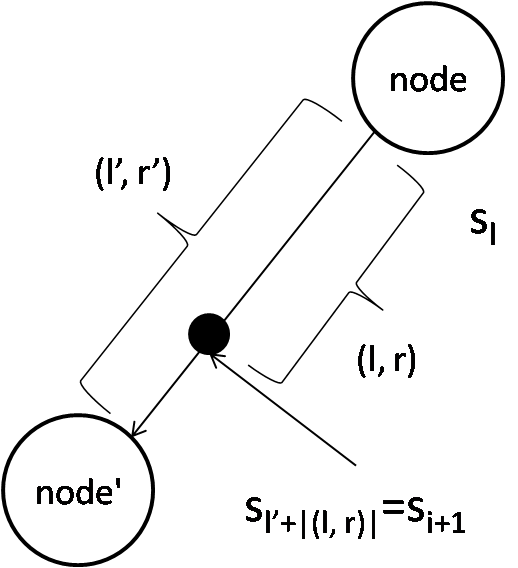
\includegraphics[scale=0.5]{img/implicit-end-point.eps}
  \caption{Implicit end point}
  \label{fig:implicit-end-point}
\end{figure}

Ukkonen finds a very important fact that if $(node, (l, i))$ is the end
point of $SuffixTree(S_i)$, then $(node, (l, i+1))$ is the active point of
$SuffixTree(S_{i+1})$.

This is because if $(node, (l, i))$ is the end point of $SuffixTree(S_i)$,
it must have a $s_{i+1}$-child (either explicitly or implicitly).
If this end point represents suffix $s_ks_{k+1}...s_i$, it is the longest
suffix in $SuffixTree(S_i)$ which satisfies $s_ks_{k+1}...s_is_{i+1}$ is a sub-string
of $S_i$. Consider $S_{i+1}$, $s_ks_{k+1}...s_is_{i+1}$ must occur at least
twice in $S_{i+1}$, so position $(node, (l, i+1))$ is the active point of
$SuffixTree(S_{i+1})$. Figure \ref{fig:ep-ap} shows about this truth.

\begin{figure}[htbp]
  \centering
  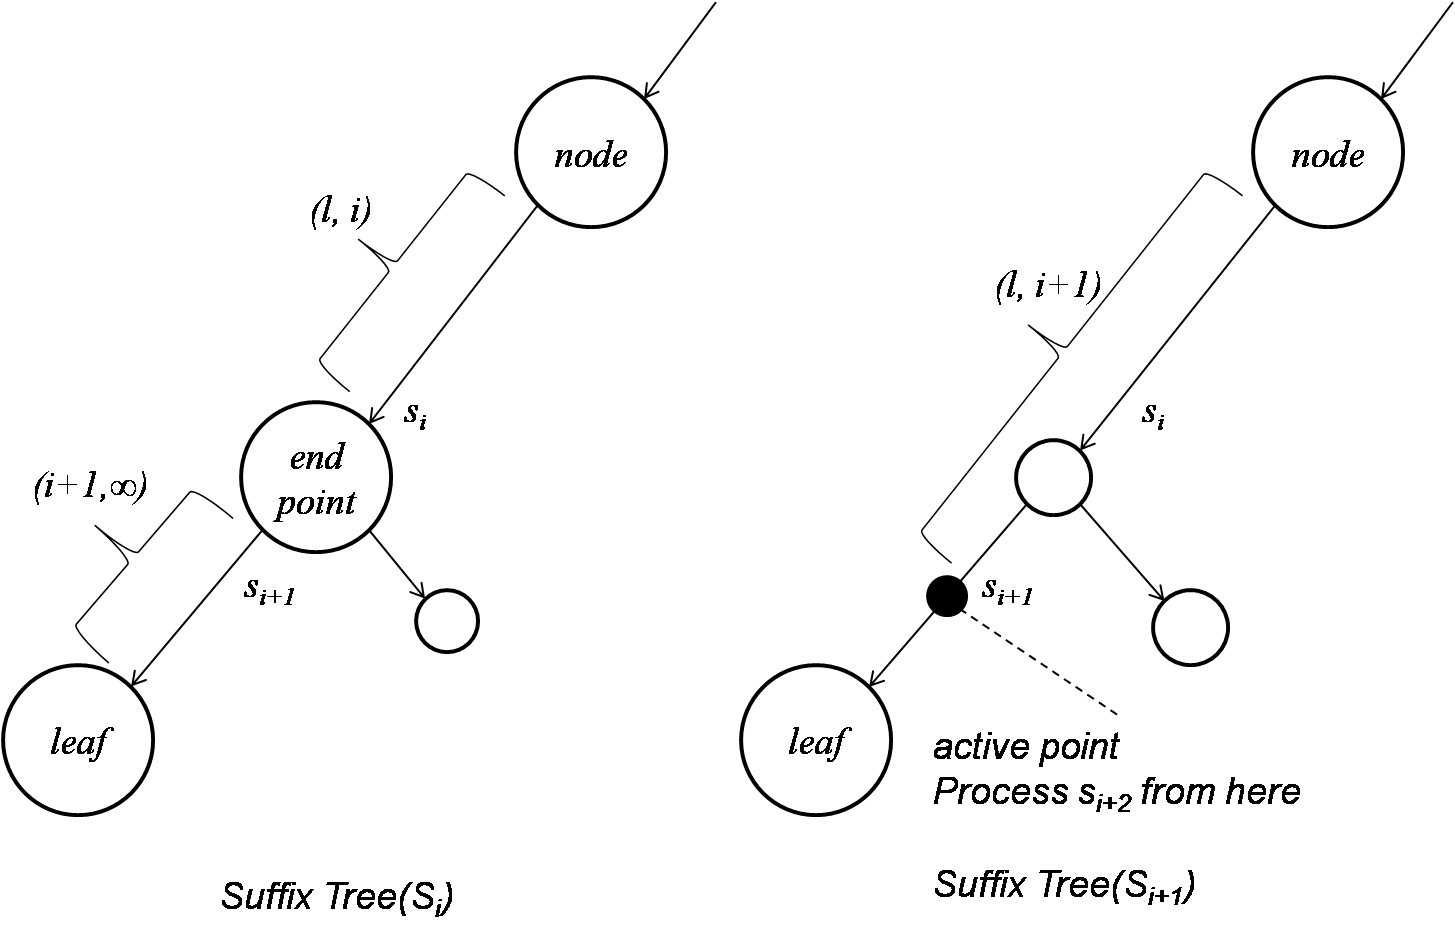
\includegraphics[scale=0.5]{img/ep-ap.eps}
  \caption{End point in $SuffixTree(S_i)$ and active point in $SuffixTree(S_{i+1})$.}
  \label{fig:ep-ap}
\end{figure}

Summarize the above facts, the algorithm of Ukkonen's on-line construction can
be given as the following.

%\begin{algorithm}
\begin{algorithmic}[1]
\Function{Update}{$node, (l, i)$}
  \State $prev \gets$ \Call{Create-Empty-Node}{} \Comment{Initialized as sentinel} %
  \Loop \Comment{Traverse along the suffix links}
    \State $(finish, node') \gets$ \Call{End-Point-Branch?}{$node, (l, i-1), s_i$}
    \If{$finish$}
      \State break
    \EndIf
    \State \Call{Children}{$node'$}[$s_i$] $\gets$ ($(i, \infty)$, \Call{Create-Empty-Node}{})
    \State \Call{Suffix-Link}{$prev$} $\gets node'$
    \State $prev \gets node'$
    \State $(node, l) = $ \textproc{Canonize}(\Call{Suffix-Link}{$node$}, $(l, i-1)$)
  \EndLoop
  \State \Call{Suffix-Link}{$prev$} $\gets node$
  \State \Return $(node, l)$ \Comment{The end point}
\EndFunction
\end{algorithmic}
%\caption{Update $SuffixTree(S_{i-1})$}
%\label{algo:update}
%\end{algorithm}

This algorithm takes reference pair $(node, (l, i))$ as arguments, note that
position $(node, (l, i-1)$ is the active point for $SuffixTree(S_{i-1})$.
Then we start a loop, this loop goes along the suffix links until
the current position $(node, (l, i-1))$ is the end point. Otherwise,
function \textproc{End-Point-Branch?} returns a position, from
where the new leaf branch out.

The \textproc{End-Point-Branch?} algorithm is realized as below.

%\begin{algorithm}
\begin{algorithmic}
\Function{End-Point-Branch?}{$node, (l, r), c$}
  \If{$(l, r) = \epsilon$}
    \If{$node = $ NIL}
      \State \Return (TRUE, $root$)
    \Else
      \State \Return (\Call{Children}{$node$}[$c$] = NIL, $node$)
    \EndIf
  \Else
    \State $((l', r'), node') \gets$ \Call{Children}{$node$}[$s_l$]
    \State $pos \gets l' + |(l, r)|$
    \If{$s_{pos} = c$}
      \State \Return (TRUE, $node$)
    \Else
      \State $p \gets$ \Call{Create-Empty-Node}{}
      \State \Call{Children}{$node$}[$s_{l'}$] $\gets ((l', pos-1), p)$
      \State \Call{Children}{$p$}[$s_{pos}$] $\gets ((pos, r'), node')$
      \State \Return (FALSE, $p$)
    \EndIf
  \EndIf
\EndFunction
\end{algorithmic}
%\caption{Test if a position is end point and create explicit node for further branching.}
%\label{algo:branch}
%\end{algorithm}

If the position is $(root, \epsilon)$, it means we have arrived at the root.
It's definitely the end point, so that we can finish this round of updating.
If the position is in form of $(node, \epsilon)$, it means the reference pair represents
an explicit node, we can examine if this node has already the $c$-child, where $c=s_i$.
If not, we need branch out a leaf.

Otherwise, the position $(node, (l, r))$ points to an implicit node.
We need find the exact position next to it to see if there is a $c$-child.
If yes, we meet an end point, the updating loop can be finished; else, we turn
the position to an explicit node, and return it for further branching.

We can finalize the Ukkonen's algorithm as below.

%\begin{algorithm}
\begin{algorithmic}[1]
\Function{Suffix-Tree}{$S$}
  \State $root \gets$ \Call{Create-Empty-Node}{}
  \State $node \gets root, l \gets 0$
  \For{$i \gets 1$ to $|S|$}
    \State $(node, l) = $ \Call{Update}{$node, (l, i)$}
    \State $(node, l) = $ \Call{Canonize}{$node, (l, i)$}
  \EndFor
  \State \Return $root$
\EndFunction
\end{algorithmic}
%\caption{Main algorithm of Ukkonen's on-line construction for suffix tree.}
%\label{algo:ukkonen2}
%\end{algorithm}

Figure \ref{fig:cons-stree-cacao} shows the steps when constructing the
suffix tree for string ``cacao''.

\begin{figure}[htbp]
  \centering
  \subfloat[Empty]{\hspace{.1\textwidth}\includegraphics[scale=0.5]{img/strie-empty.ps}\hspace{.1\textwidth}}
  \subfloat[``c'']{\hspace{.1\textwidth}\includegraphics[scale=0.5]{img/stree-c.ps}\hspace{.1\textwidth}}
  \subfloat[``ca'']{\hspace{.1\textwidth}\includegraphics[scale=0.5]{img/stree-ca.ps}\hspace{.1\textwidth}} \\
  \subfloat[``cac'']{\hspace{.1\textwidth}\includegraphics[scale=0.5]{img/stree-cac.ps}\hspace{.1\textwidth}}
  \subfloat[``caca'']{\hspace{.1\textwidth}\includegraphics[scale=0.5]{img/stree-caca.ps}\hspace{.1\textwidth}}
  \subfloat[``cacao'']{\hspace{.1\textwidth}\includegraphics[scale=0.5]{img/stree-cacao.ps}\hspace{.1\textwidth}}
  \caption{Construct suffix tree for ``cacao''. There are 6 steps. Only the last layer of suffix links are shown in dotted arrow.}
  \label{fig:cons-stree-cacao}
\end{figure}

Note that we needn't set suffix link for leaf nodes, only branch nodes
need suffix links.

The following example Python program implements Ukkonen's algorithm.
First is the node definition.

\lstset{language=Python}
\begin{lstlisting}
class Node:
    def __init__(self, suffix=None):
        self.children = {} # 'c':(word, Node), where word = (l, r)
        self.suffix = suffix
\end{lstlisting}

Because there is only one copy of the complete string, all sub-strings
are represent in $(left, right)$ pairs, and the leaf are open pairs
as $(left, \infty)$. The suffix tree is defined like below.

\begin{lstlisting}
class STree:
    def __init__(self, s):
        self.str = s
        self.infinity = len(s)+1000
        self.root = Node()
\end{lstlisting}

The infinity is defined as the length of the string plus a big number.
Some auxiliary functions are defined.

\begin{lstlisting}
def substr(str, str_ref):
    (l, r)=str_ref
    return str[l:r+1]

def length(str_ref):
    (l, r)=str_ref
    return r-l+1
\end{lstlisting}

The main entry for Ukkonen's algorithm is implemented as the following.

\begin{lstlisting}
def suffix_tree(str):
    t = STree(str)
    node = t.root # init active point is (root, Empty)
    l = 0
    for i in range(len(str)):
        (node, l) = update(t, node, (l, i))
        (node, l) = canonize(t, node, (l, i))
    return t

def update(t, node, str_ref):
    (l, i) = str_ref
    c = t.str[i] # current char
    prev = Node() # dummy init
    while True:
        (finish, p) = branch(t, node, (l, i-1), c)
        if finish:
            break
        p.children[c]=((i, t.infinity), Node())
        prev.suffix = p
        prev = p
        (node, l) = canonize(t, node.suffix, (l, i-1))
    prev.suffix = node
    return (node, l)

def branch(t, node, str_ref, c):
    (l, r) = str_ref
    if length(str_ref)<=0: # (node, empty)
        if node is None: #_|_
            return (True, t.root)
        else:
            return ((c in node.children), node)
    else:
        ((l1, r1), node1) = node.children[t.str[l]]
        pos = l1+length(str_ref)
        if t.str[pos]==c:
            return (True, node)
        else:
            branch_node = Node()
            node.children[t.str[l1]]=((l1, pos-1), branch_node)
            branch_node.children[t.str[pos]] = ((pos, r1), node1)
            return (False, branch_node)

def canonize(t, node, str_ref):
    (l, r) = str_ref
    if node is None:
        if length(str_ref)<=0:
            return (None, l)
        else:
            return canonize(t, t.root, (l+1, r))
    while l<=r: # str_ref is not empty
        ((l1, r1), child) = node.children[t.str[l]]
        if r-l >= r1-l1:
            l += r1-l1+1
            node = child
        else:
            break
    return (node, l)
\end{lstlisting}

\subsubsection{Functional suffix tree construction}
\index{Suffix tree!functional construction}

Giegerich and Kurtz found Ukkonen's algorithm
can be transformed to McCreight's algorithm\cite{GieKur97}.
The three suffix tree construction algorithms found by
Weiner, McCreight, and Ukkonen are all bound to $O(n)$ time.
Giegerich and Kurtz conjectured any sequential
suffix tree construction method doesn't base on
suffix links, active suffixes, etc., fails to meet the
$O(n)$-criterion.

There is implementation in PLT/Scheme\cite{plt-stree} based on
Ukkonen's algorithm, However, it updates suffix links during the
processing, which is not purely functional.

A lazy suffix tree construction method is discussed in \cite{GieKur95}.
And this method is contributed to Haskell Hackage by Bryan O'Sullivan.
\cite{Hackage-STree}. The method depends on the lazy evaluation property.
The tree won't be constructed until it is traversed.
However, it can't ensure the $O(n)$ performance
if the programming environments or languages don't support
lazy evaluation.

The following Haskell program defines the suffix tree. A suffix tree
is either a leaf, or a branch containing multiple sub trees. Each
sub tree is bound to a string.

\lstset{language=Haskell}
\begin{lstlisting}
data Tr = Lf | Br [(String, Tr)] deriving (Eq)
type EdgeFunc = [String]->(String, [String])
\end{lstlisting}

The edge function extracts a common prefix from a list of strings.
The prefix returned by edge function may not be the longest one,
empty string is also allowed. The exact behavior can be customized
with different edge functions.

\[
build(edge, X)
\]

This defines a generic radix tree building function. It takes an
edge function, and a set of strings. $X$ can be all suffixes of
a string, so that we get suffix trie or suffix tree. We'll also
explain later that $X$ can be all prefixes, which lead to normal
prefix trie or Patricia.

Suppose all the strings are built from a character set $\Sigma$.
When build the tree, if the string is empty, $X$ only contains
one empty string as well. The result tree is an empty leaf;
Otherwise, we examine every character in $\Sigma$, group
the strings in $X$ with their initial characters, the apply
the edge function to these groups.

\be
build(edge, X) = \left \{
  \begin{array}
  {r@{\quad:\quad}l}
  leaf & X = \{ \phi \} \\
  \begin{array}{ll}
    branch(\{(\{c\} \cup p, & build(edge, X')) | \\
                            & c \in \Sigma, \\
                            & G \in \{ group(X, c) \}, \\
                            & (p, X') \in \{ edge(G) \} \})
  \end{array} & otherwise
  \end{array}
\right.
\ee

The algorithm categorizes all suffixes by the
first letter in several groups. It removes the first letter for each element in every group.
For example, the suffixes $\{$``acac'', ``cac'', ``ac'', ``c''$\}$ are
categorized to groups $\{$('a', [``cac'', ``c'']), ('c', [``ac'', ``''])$\}$.

\be
group(X, c) = \{C' | \{c_1\} \cup C' \in X, c_1 = c\}
\ee

Function $group$ enumerates all suffixes in $X$, for each one, denote the first
character as $c_1$, the rest characters as $C'$. If $c_1$ is same as
the given character $c$, then $C'$ is collected.

Below example Haskell program implements the generic radix tree building algorithm.

\begin{lstlisting}
alpha = ['a'..'z']++['A'..'Z']

lazyTree::EdgeFunc -> [String] -> Tr
lazyTree edge = build where
    build [[]] = Lf
    build ss = Br [(a:prefix, build ss') |
                         a<-alpha,
                         xs@(x:_) <-[[cs | c:cs<-ss, c==a]],
                         (prefix, ss')<-[edge xs]]
\end{lstlisting}

Different edge functions produce different radix trees. Since edge function
extracts common prefix from a set of strings. The simplest one constantly
uses the empty string as the common prefix. This edge function builds a trie.

\be
edgeTrie(X) = (\phi, X)
\ee

We can also realize an edge function, that extracts the longest common prefix.
Such edge function builds a Patricia.
Denote the strings as $X = \{x_1, x_2, ..., x_n\}$, for the each string $x_i$,
let the initial character be $c_i$, and the rest characters in $x_i$ as $W_i$.
If there is only one string in $X$, the longest common prefix is definitely
this string; If there are two strings start with different initial characters,
the longest common prefix is empty; Otherwise,it means all the strings
share the same initial character. This character definitely belongs to
the longest common prefix. We can remove it from all strings, and recursively
call the edge function.

\be
edgeTree(X) = \left \{
  \begin{array}
  {r@{\quad:\quad}l}
  (x_1, \{ \phi \}) & X = \{ x_1 \} \\
  (\phi, X) & |X| > 1, \exists x_i \in X, c_i \neq c_1 \\
  (\{c_1\} \cup p, Y) & (p, Y) = edgeTree(\{ W_i | x_i \in X \})
  \end{array}
\right.
\ee

Here are some examples for $edgeTree$ function.
\[
\begin{array}{l}
edgeTree(\{ \text{``an'', ``another'', ``and''}\}) = (\text{``an''}, \{\text{``'', ``other'', ``d''}\}) \\
edgeTree(\{ \text{``bool'', ``foo, ``bar''}\}) = (\text{``''}, \{\text{``bool'', ``fool'', ``bar''}\})
\end{array}
\]

The following example Haskell program implements this edge function.

\begin{lstlisting}
edgeTree::EdgeFunc
edgeTree [s] = (s, [[]])
edgeTree awss@((a:w):ss) | null [c|c:_<-ss, a/=c] = (a:prefix, ss')
                         | otherwise              = ("", awss)
                         where (prefix, ss') = edgeTree (w:[u| _:u<-ss])
edgeTree ss = ("", ss)
\end{lstlisting}

For any given string, we can build suffix trie and suffix tree by feeding suffixes to these
two edge functions.

\be
suffixTrie(S) = build(edgeTrie, suffixes(S))
\ee

\be
suffixTree(S) = build(edgeTree, suffixes(S))
\ee

Because the $build(edge, X)$ is generic, it can be used to build other radix trees, such
as the normal prefix trie and Patricia.

\be
trie(S) = build(edgeTrie, prefixes(S))
\ee

\be
tree(S) = build(edgeTree, prefixes(S))
\ee

% ================================================================
%               Suffix tree applications
% ================================================================

\section{Suffix tree applications}

Suffix tree can help to solve many string and DNA pattern manipulation problems
particularly fast.

\subsection{String/Pattern searching}
\label{substring-lookup}
\index{Suffix tree!string searching}

There a plenty of string searching algorithms, such as the
famous KMP(Knuth-Morris-Pratt algorithm is introduced in the chapter of search)
algorithm. Suffix tree can perform at the same level as
KMP\cite{zhang-shaojie-lec}. the string searching in bound to $O(m)$ time,
where $m$ is the length of the sub-string to be search. However, $O(n)$ time is
required to build the suffix tree in advance, where $n$ is the length
of the text\cite{lallison-stree}.

Not only sub-string searching, but also pattern matching, including
regular expression matching can be solved with suffix tree. Ukkonen
summarizes this kind of problems as sub-string motifs:
{\em For a string $S$, $SuffixTree(S)$ gives complete occurrence
counts of all sub-string motifs of $S$ in $O(n)$ time, although $S$ may have
$O(n^2)$ sub-strings.}

\subsubsection{Find the number of sub-string occurrence}
\index{Suffix tree!sub-string occurrence}

Every internal node in $SuffixTree(S)$ is corresponding
to a sub-string occurs multiple times in $S$. If this sub-string occurs
$k$ times in $S$, then there are total $k$ sub-trees under this node\cite{ukkonen-lec}.

\begin{algorithmic}[1]
\Function{Lookup-Pattern}{$T, s$}
  \Loop
    \State $match \gets$ FALSE
    \For{$\forall (s_i, T_i) \in$ \textproc{Values}(\Call{Children}{$T$})}
      \If{$s \sqsubset s_i$}
        \State \Return \textproc{Max}($|$\Call{Children}{$T_i$}$|$, 1)
      \ElsIf{$s_i \sqsubset s$}
        \State $match \gets$ TRUE
        \State $T \gets T_i$
        \State $s \gets s - s_i$
        \State break
      \EndIf
    \EndFor
    \If{$\lnot match$}
      \State \Return 0
    \EndIf
  \EndLoop
\EndFunction
\end{algorithmic}

When look up a sub-string pattern $s$ in text $w$, we build the suffix tree $T$ from the
text. Start from the root, we iterate all children. For every
string reference pair $s_i$ and sub-tree $T_i$, we check if the $s$ is prefix of $s_i$.
If yes, the number of sub-trees in $T_i$ is returned as the result.
There is a special case that $T_i$ is a leaf without any children. We need return 1 but
not zero. This is why we use the maximum function.
Otherwise, if $s_i$ is prefix of $s$, then we remove $s_i$ part from $s$, and recursively
look up in $T_i$.

The following Python program implements this algorithm.

\lstset{language=Python}
\begin{lstlisting}
def lookup_pattern(t, s):
    node = t.root
    while True:
        match = False
        for _, (str_ref, tr) in node.children.items():
            edge = substr(t, str_ref)
            if string.find(edge, s)==0: #s `isPrefixOf` edge
                return max(len(tr.children), 1)
            elif string.find(s, edge)==0: #edge `isPrefixOf` s
                match = True
                node = tr
                s = s[len(edge):]
                break
        if not match:
            return 0
    return 0 # not found
\end{lstlisting}

This algorithm can also be realized in recursive way. For the non-leaf
suffix tree $T$, denote the children as $C = \{(s_1, T_1), (s_2, T_2), ...\}$.
We search the sub string among the children.

\be
lookup_{pattern}(T, s) = find(C, s)
\ee

If children $C$ is empty, it means the sub string doesn't occurs at all.
Otherwise, we examine the first pair $(s_1, T_1)$, if $s$ is prefix of $s_1$,
then the number of sub-trees in $T_1$ is the result. If $s_1$ is prefix
of $s$, we remove $s_1$ from $s$, and recursively look up it in $T_1$;
otherwise, we go on to examine the rest children denoted as $C'$.

\be
find(C, s) = \left \{
  \begin{array}
  {r@{\quad:\quad}l}
  0 & C = \phi \\
  max(1, |C_1|) & s \sqsubset s_1 \\
  lookup_{pattern}(T_1, s - s_1) & s_1 \sqsubset s \\
  find(C', s) & otherwise
  \end{array}
\right.
\ee

The following Haskell example code implements this algorithm.

\lstset{language=Haskell}
\begin{lstlisting}
lookupPattern (Br lst) ptn = find lst where
    find [] = 0
    find ((s, t):xs)
         | ptn `isPrefixOf` s = numberOfBranch t
         | s `isPrefixOf` ptn = lookupPattern t (drop (length s) ptn)
         | otherwise = find xs
    numberOfBranch (Br ys) = length ys
    numberOfBranch _ = 1

findPattern s ptn = lookupPattern (suffixTree $ s++"$") ptn
\end{lstlisting}

We always append special terminator to the string (the `\$' in above program),
so that there won't be any suffix becomes the prefix of the other\cite{wiki-suffix-tree}.

Suffix tree also supports searching pattern like ``a**n'', we skip it here.
Readers can refer to \cite{ukkonen-lec} and \cite{ukkonen-search} for details.

\subsection{Find the longest repeated sub-string}
\index{Longest repeated sub-string}

{\em After adding a special terminator character to string S, The
longest repeated sub-string can be found by searching the
deepest branches in suffix tree.}

Consider the example suffix tree shown in figure \ref{fig:stree-mississippis}

\begin{figure}[htbp]
  \centering
  \includegraphics[scale=0.5]{img/stree-mississippis.ps}
  \caption{The suffix tree for `mississippi\$'} \label{fig:stree-mississippis}
\end{figure}

There are three branch nodes, $A$, $B$, and $C$ with depth 3. However, $A$ represents
the longest repeated sub-string ``issi''. $B$ and $C$ represent for ``si'', ``ssi'',
they are shorter than $A$.

This example tells us that the ``depth'' of the branch node should be measured
by the number of characters traversed from the root. But not the number of
explicit branch nodes.

To find the longest repeated sub-string, we can perform BFS in the suffix tree.

\begin{algorithmic}[1]
\Function{Longest-Repeated-Substring}{$T$}
  \State $Q \gets$ (NIL, \Call{Root}{$T$})
  \State $R \gets$ NIL
  \While{$Q$ is not empty}
    \State $(s, T) \gets$ \Call{Pop}{$Q$}
    \For{each $((l, r), T') \in$ \Call{Children}{$T$}}
      \If{$T'$ is not leaf}
        \State $s' \gets$ \Call{Concatenate}{$s, (l, r)$}
        \State \Call{Push}{$Q, (s', T')$}
        \State $R \gets$ \Call{Update}{$R, s'$}
      \EndIf
    \EndFor
  \EndWhile
  \State \Return $R$
\EndFunction
\end{algorithmic}

This algorithm initializes a queue with a pair of an
empty string and the root. Then it repeatedly examine the candidate in the queue.

For each node, the algorithm examines each children one by one.
If it is a branch node, the child is pushed back
to the queue for further search. And the sub-string represented
by this child will be treated as a candidate of the
longest repeated sub-string.

Function \textproc{Update}($R, s'$) updates the longest repeated
sub-string candidates. If multiple candidates have the same length, they
are all kept in a result list.

\begin{algorithmic}[1]
\Function{Update}{$L, s$}
  \If{$L =$ NIL $\lor |l_1| < |s|$}
    \State \Return $l \gets \{ s \}$
  \EndIf
  \If {$|l_1| = |s|$}
    \State \Return \Call{Append}{$L, s$}
  \EndIf
  \State \Return $L$
\EndFunction
\end{algorithmic}

The above algorithm can be implemented in Python as the following example program.

\lstset{language=Python}
\begin{lstlisting}
def lrs(t):
    queue = [("", t.root)]
    res = []
    while len(queue)>0:
        (s, node) = queue.pop(0)
        for _, (str_ref, tr) in node.children.items():
            if len(tr.children)>0:
                s1 = s+t.substr(str_ref)
                queue.append((s1, tr))
                res = update_max(res, s1)
    return res

def update_max(lst, x):
    if lst ==[] or len(lst[0]) < len(x):
        return [x]
    if len(lst[0]) == len(x):
        return lst + [x]
    return lst
\end{lstlisting}

Searching the deepest branch can also be realized recursively.
If the tree is just a leaf node, empty string is returned, else the
algorithm tries to find the longest repeated sub-string from the
children.

\be
LRS(T) = \left \{
  \begin{array}
  {r@{\quad:\quad}l}
  \phi & leaf(T) \\
  longest(\{s_i \cup LRS(T_i) | (s_i, T_i) \in C, \lnot leaf(T_i)\}) & otherwise
  \end{array}
\right.
\ee

The following Haskell example program implements the longest repeated sub-string algorithm.
\lstset{language=Haskell}
\begin{lstlisting}
isLeaf Lf = True
isLeaf _ = False

lrs'::Tr->String
lrs' Lf = ""
lrs' (Br lst) = find $ filter (not . isLeaf . snd) lst where
    find [] = ""
    find ((s, t):xs) = maximumBy (compare `on` length) [s++(lrs' t), find xs]
\end{lstlisting} %$

\subsection{Find the longest common sub-string}
\index{Longest common sub-string}

The longest common sub-string, can also be quickly found
with suffix tree. The solution is to build a generalized suffix
tree. If the two strings are denoted as $txt_1$ and
$txt_2$, a generalized suffix tree is $SuffixTree(txt_1\$_1txt_2\$_2)$.
Where $\$_1$ is a special terminator character for $txt_1$, and
$\$_2 \neq \$_1$ is another special terminator character for $txt_2$.

The longest common sub-string is indicated by the deepest branch node, with
two forks corresponding to both ``...$\$_1$...'' and ``...$\$_2$''(no $\$_1$).
The definition of the {\em deepest} node is as same as the one for
the longest repeated sub-string, it is the number of characters traversed
from root.

If a node has ``...$\$_1$...'' under it, the node must represent
a sub-string of $txt_1$, as $\$_1$ is the terminator of $txt_1$.
On the other hand, since it also has ``...$\$_2$'' (without $\$_1$), this node
must represent a sub-string of $txt_2$ too. Because it's the deepest
one satisfied this criteria, so the node represents the longest common
sub-string.

Again, we can use BFS (bread first search) to find the longest common sub-string.

\begin{algorithmic}[1]
\Function{Longest-Common-Substring}{$T$}
  \State $Q \gets$ (NIL, \Call{Root}{$T$})
  \State $R \gets$ NIL
  \While{$Q$ is not empty}
    \State $(s, T) \gets$ \Call{POP}{$Q$}
    \If{\Call{Match-Fork}{$T$}}
      \State $R \gets$ \Call{Update}{$R, s$}
    \EndIf
    \For{each $((l, r), T') \in $ \Call{Children}{$T$}}
      \If{$T'$ is not leaf}
        \State $s' \gets$ \Call{Concatenate}{$s, (l, r)$}
        \State \Call{Push}{$Q, (s', T')$}
      \EndIf
    \EndFor
  \EndWhile
  \State \Return $R$
\EndFunction
\end{algorithmic}

Most part is as same as the the longest repeated sub-sting searching algorithm.
The function \text{Match-Fork} checks if the children satisfy the common sub-string criteria.

\begin{algorithmic}[1]
\Function{Match-Fork}{$T$}
  \If{$|$ \Call{Children}{$T$} $| = 2$}
    \State $\{(s_1, T_1), (s_2, T_2)\} \gets$ \Call{Children}{$T$}
    \State \Return $T_1$ is leaf $\land T_2$ is leaf $\land$ \Call{Xor}{$\$_1 \in s_1, \$_1 \in s_2)$}
  \EndIf
  \State \Return FALSE
\EndFunction
\end{algorithmic}

In this function, it checks if the two children
are both leaf. One contains $\$_2$, while the
other doesn't. This is because
if one child is a leaf, it always contains $\$_1$
according to the definition of suffix tree.

The following Python program implement the longest common sub-string program.

\lstset{language=Python}
\begin{lstlisting}
def lcs(t):
    queue = [("", t.root)]
    res = []
    while len(queue)>0:
        (s, node) = queue.pop(0)
        if match_fork(t, node):
            res = update_max(res, s)
        for _, (str_ref, tr) in node.children.items():
            if len(tr.children)>0:
                s1 = s + t.substr(str_ref)
                queue.append((s1, tr))
    return res

def is_leaf(node):
    return node.children=={}

def match_fork(t, node):
    if len(node.children)==2:
        [(_, (str_ref1, tr1)), (_, (str_ref2, tr2))]=node.children.items()
        return is_leaf(tr1) and is_leaf(tr2) and
            (t.substr(str_ref1).find('#')!=-1) !=
            (t.substr(str_ref2).find('#')!=-1)
    return False
\end{lstlisting}

The longest common sub-string finding algorithm can also be
realized recursively. If the suffix tree $T$ is a leaf, the result is empty;
Otherwise, we examine all children in $T$. For those satisfy the matching
criteria, the sub-string are collected as candidates; for those don't
matching, we recursively search the common sub-string among the children.
The longest candidate is selected as the final result.

\be
LCS(T) = \left \{
  \begin{array}
  {r@{\quad:\quad}l}
  \phi & leaf(T) \\
  \begin{array}{ll}
    longest( & \{s_i | (s_i, T_i) \in C, match(T_i)\} \cup \\
             & \{s_i \cup LCS(T_i) | (s_i, T_i) \in C, \lnot match(T_i)\})
  \end{array} & otherwise
  \end{array}
\right.
\ee

The following Haskell example program implements the longest common sub-string algorithm.

\lstset{language=Haskell}
\begin{lstlisting}
lcs Lf = []
lcs (Br lst) = find $ filter (not .isLeaf . snd) lst where
    find [] = []
    find ((s, t):xs) = maxBy (compare `on` length)
                       (if match t
                        then s:(find xs)
                        else  (map (s++) (lcs t)) ++ (find xs))

match (Br [(s1, Lf), (s2, Lf)]) = ("#" `isInfixOf` s1) /= ("#" `isInfixOf` s2)
match _ = False
\end{lstlisting}

\subsection{Find the longest palindrome}
\index{Longest palindrome}

A palindrome is a string, $S$, such that $S=reverse(S)$ For example,
``level'', ``rotator'', ``civic'' are all palindrome.

The longest palindrome in a string $s_1s_2...s_n$ can be found in
$O(n)$ time with suffix tree. The solution can be benefit from the
longest common sub-string algorithm.

For string $S$, if sub-string $w$ is a palindrome, then it must be
sub-string of $reverse(S)$ too. for instance, ``issi'' is a palindrome,
it is a sub-string of ``mississippi''. When reverse to
``ippississim'', ``issi'' is also a sub-string.

Based on this fact, we can find the longest palindrome by
searching the longest common sub-string for $S$ and $reverse(S)$.

\be
palindrome_m(S) = LCS(suffixTree(S \cup reverse(S)))
\ee

The following Haskell example program finds the longest palindrome.

\lstset{language=Haskell}
\begin{lstlisting}
longestPalindromes s = lcs $ suffixTree (s++"#"++(reverse s)++"$")
\end{lstlisting}

\subsection{Others}
Suffix tree can also be used for data compression, such as Burrows-Wheeler
transform, LZW compression (LZSS) etc. \cite{wiki-suffix-tree}

% ================================================================
%                 Short summary
% ================================================================
\section{Notes and short summary}

Suffix Tree was first introduced by Weiner in 1973 \cite{weiner}.
In 1976, McCreight greatly simplified the construction algorithm.
McCreight constructs the suffix tree from right to left. In 1995,
Ukkonen gave the first on-line construction algorithms from
left to right. All the three algorithms are linear time ($O(n)$).
And some research shows the relationship among these 3 algorithms.
\cite{GieKur97}

\begin{thebibliography}{99}

\bibitem{ukkonen95}
Esko Ukkonen. ``On-line construction of suffix trees''. Algorithmica 14 (3): 249--260. doi:10.1007/BF01206331. http://www.cs.helsinki.fi/u/ukkonen/SuffixT1withFigs.pdf

\bibitem{weiner73}
Weiner, P. ``Linear pattern matching algorithms'', 14th Annual IEEE Symposium on Switching and Automata Theory, pp. 1-11, doi:10.1109/SWAT.1973.13

\bibitem{wiki-suffix-tree}
Suffix Tree, Wikipedia. http://en.wikipedia.org/wiki/Suffix\_tree

\bibitem{ukkonen-presentation}
Esko Ukkonen. ``Suffix tree and suffix array techniques for pattern analysis in strings''. http://www.cs.helsinki.fi/u/ukkonen/Erice2005.ppt

\bibitem{wiki-trie}
Trie, Wikipedia. http://en.wikipedia.org/wiki/Trie

\bibitem{trivial-stree-java}
Suffix Tree (Java). http://en.literateprograms.org/Suffix\_tree\_(Java)

\bibitem{GieKur97}
Robert Giegerich and Stefan Kurtz. ``From Ukkonen to McCreight and Weiner: A Unifying View of Linear-Time Suffix Tree Construction''. Science of Computer Programming 25(2-3):187-218, 1995. http://citeseer.ist.psu.edu/giegerich95comparison.html

\bibitem{GieKur95}
Robert Giegerich and Stefan Kurtz. ``A Comparison of Imperative and Purely Functional Suffix Tree Constructions''. Algorithmica 19 (3): 331--353. doi:10.1007/PL00009177. www.zbh.uni-hamburg.de/pubs/pdf/GieKur1997.pdf

\bibitem{Hackage-STree}
Bryan O'Sullivan. ``suffixtree: Efficient, lazy suffix tree implementation''. http://hackage.haskell.org/package/suffixtree

\bibitem{plt-stree}
Danny. http://hkn.eecs.berkeley.edu/~dyoo/plt/suffixtree/

\bibitem{zhang-shaojie-lec}
Zhang Shaojie. ``Lecture of Suffix Trees''. http://www.cs.ucf.edu/~shzhang/Combio09/lec3.pdf

\bibitem{lallison-stree}
Lloyd Allison. ``Suffix Trees''. http://www.allisons.org/ll/AlgDS/Tree/Suffix/

\bibitem{ukkonen-lec}
Esko Ukkonen. ``Suffix tree and suffix array techniques for pattern analysis in strings''. http://www.cs.helsinki.fi/u/ukkonen/Erice2005.ppt

\bibitem{ukkonen-search}
Esko Ukkonen ``Approximate string-matching over suffix trees''. Proc. CPM 93. Lecture Notes in Computer Science 684, pp. 228-242, Springer 1993. http://www.cs.helsinki.fi/u/ukkonen/cpm931.ps

\end{thebibliography}

\ifx\wholebook\relax \else
\end{document}
\fi
